
LLVM is an enormous software, with hundreds of components working closely together. Its ever-increasing running time is slowly becoming an issue. This affects many use cases that are sensitive to compilation time—for example, the Just-in-Time (JIT) compiler. To diagnose this problem in a systematic way, LLVM provides some useful utilities for profiling the execution time.

Time profiling has always been an important topic in software development. With the running time collected from individual software components, we can spot performance bottlenecks more easily. In this section, we are going to learn about two tools provided by LLVM: the Timer class and the TimeTraceScope class. Let's start with the Timer class first.

\subsubsubsection{11.4.1\hspace{0.2cm}Using the Timer class}

The Timer class, as suggested by its name, can measure the execution time of a code region. Here is an example of this:

\begin{lstlisting}[style=styleCXX]
#include "llvm/Support/Timer.h"
…
Timer T("MyTimer", "A simple timer");
T.startTimer();
// Do some time-consuming works…
T.stopTimer();
\end{lstlisting}

In the preceding snippet, Timer instance T measures the time spent in the region, enclosed by the startTimer and stopTimer method calls. 

Now that we have collected the timing data, let's try to print it out. Here is an example of this:

\begin{lstlisting}[style=styleCXX]
Timer T(…);
…
TimeRecord TR = T.getTotalTime();
TR.print(TR, errs());
\end{lstlisting}

In the previous code snippet, a TimeRecord instance encapsulates the data collected by the Timer class. We can then use TimeRecord::print to print it to a stream—in this case, the errs() stream. In addition, we assigned another TimeRecord instance—via the first argument of print—as the total time interval we want to compare it against. Let's look at the output of this code, as follows:

\begin{tcblisting}{commandshell={}}
===---------------------------------------------------------===
                Miscellaneous Ungrouped Timers
===---------------------------------------------------------===
---User Time--- --User+System-- ---Wall Time--- ---Name ---
 0.0002 (100.0%) 0.0002 (100.0%) 0.0002 (100.0%) A simple timer
 0.0002 (100.0%) 0.0002 (100.0%) 0.0002 (100.0%)   Total
 0.0002 (100.0%) 0.0002 (100.0%) 0.0002 (100.0%)
\end{tcblisting}

In the preceding output, the first row shows the TimeRecord instance collected from our previous Timer instance, whereas the second row shows the total time—the first argument of TimeRecord::print. 

We now know how to print the timing data collected by a single Timer instance, but what about multiple timers? LLVM provides another support utility for the Timer class: the TimerGroup class. Here's an example usage of the TimerGroup class:

\begin{lstlisting}[style=styleCXX]
TimerGroup TG("MyTimerGroup", "My collection of timers");

Timer T("MyTimer", "A simple timer", TG);
T.startTimer();
// Do some time-consuming works…
T.stopTimer();

Timer T2("MyTimer2", "Yet another simple timer", TG);
T2.startTimer();
// Do some time-consuming works…
T2.stopTimer();

TG.print(errs());
\end{lstlisting}

In the preceding code snippet, we declare a TimerGroup instance, TG, and use it as the third constructor argument for each Timer instance we create. Finally, we print them using TimerGroup::print. Here is the output of this code:

\begin{tcblisting}{commandshell={}}
===---------------------------------------------------------===
                    My collection of timers
===---------------------------------------------------------===
Total Execution Time: 0.0004 seconds (0.0004 wall clock)
  ---User Time--- --User+System-- ---Wall Time--- ---Name ---
  0.0002 ( 62.8%) 0.0002 ( 62.8%) 0.0002 ( 62.8%) A simple timer
  0.0001 ( 37.2%) 0.0001 ( 37.2%) 0.0001 ( 37.2%) Yet another simple timer
  0.0004 (100.0%) 0.0004 (100.0%) 0.0004 (100.0%) Total
\end{tcblisting}

Each row in the output (except the last one) is the TimeRecord instance for each Timer instance in this group.

So far, we have been using Timer::startTimer and Timer::stopTimer to toggle the timer. To make measuring the time interval within a code block—namely, the region enclosed with curly brackets \{\}—easier without manually calling those two methods, LLVM provides another utility that automatically starts the timer upon entering a code block and turns it off when exiting. Let's see how to use the TimeRegion class with the following sample code:

\begin{lstlisting}[style=styleCXX]
TimerGroup TG("MyTimerGroup", "My collection of timers");
{
	Timer T("MyTimer", "A simple timer", TG);
	TimeRegion TR(T);
	// Do some time-consuming works…
} {
	Timer T("MyTimer2", "Yet another simple timer", TG);
	TimeRegion TR(T);
	// Do some time-consuming works…
}

TG.print(errs());
\end{lstlisting}


As you can see in the preceding snippet, instead of calling startTimer/stopTimer, we put the to-be-measured code into a separate code block and use a TimeRegion variable to automatically toggle the timer. This code will print out the same content as the previous example. With the help of TimeRegion, we can have a more concise syntax and avoid any mistakes where we forget to turn off the timer.

You have now learned how to use Timer and its supporting utilities to measure the execution time of a certain code region. In the next section, we are going to learn a more advanced form of time measurement that captures the hierarchical structure of the program.


\subsubsubsection{11.4.2\hspace{0.2cm}Collecting the time trace}

In the previous section, we learned how to use Timer to collect the execution time of a small range of code regions. Although that gave us a portrait of the compiler's runtime performance, we sometimes need a more structural timing profile in order to fully understand any systematic issues.

TimeTraceScope is a class provided by LLVM to perform global-scope time profiling. Its usage is pretty simple: similar to TimeRegion, which we saw in the previous section, a TimeTraceScope instance automatically turns the time profiler on and off upon entering and exiting a code block. Here is an example of this:

\begin{lstlisting}[style=styleCXX]
TimeTraceScope OuterTimeScope("TheOuterScope");
for (int i = 0; i < 50; ++i) {
	{
		TimeTraceScope InnerTimeScope("TheInnerScope");
		foo();
	}
	bar();
}
\end{lstlisting}

In the preceding code snippet, we create two TimeTraceScope instances: OuterTimeScope and InnerTimeScope. These try to profile the execution time of the whole region and the time spent on function foo, respectively.

Normally, if we use Timer rather than TimeTraceScope, it can only give us the aggregate duration collected from each timer. However, in this case, we are more interested in how different parts of the code allocate themselves on the timeline. For example, does the foo function always spend the same amount of time ion every loop iteration? If that's not the case, which iterations spend more time than others?

To see the result, we need to add additional command-line options to the opt command when running the Pass (assuming you use TimeTraceScope within a Pass). Here is an example of this:

\begin{tcblisting}{commandshell={}}
$ opt –passes="…" -time-trace -time-trace-file=my_trace.json …
\end{tcblisting}

The additional -time-trace flag is asking opt to export all the traces collected by TimeTraceScope to the file designated by the -time-trace-file option.

After running this command, you will get a new file, my\_trace.json. The content of this file is basically non-human-readable, but guess what? You can visualize it using the Chrome web browser. Here are the steps to do this:

\begin{enumerate}
\item Open your Chrome web browser and type in chrome://tracing in the Uniform Resource Locator (URL) bar. You will see an interface that looks like this:

\hspace*{\fill} \\ %插入空行
\begin{center}
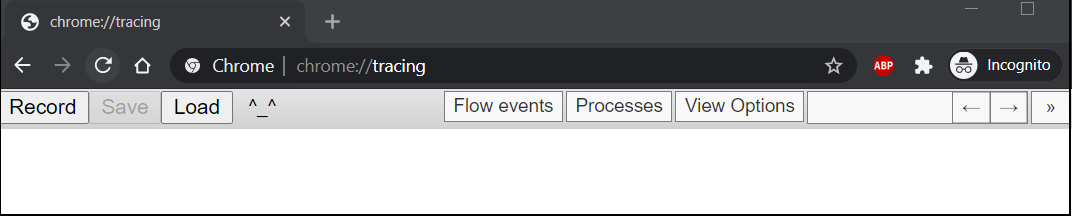
\includegraphics[width=0.9\textwidth]{content/3/chapter11/images/3.png}\\
Figure 11.3 – The trace visualizer in Chrome
\end{center}

\item Click on the Load button in the top-left corner and select our my\_trace.json file. You will see a page like this:

\hspace*{\fill} \\ %插入空行
\begin{center}
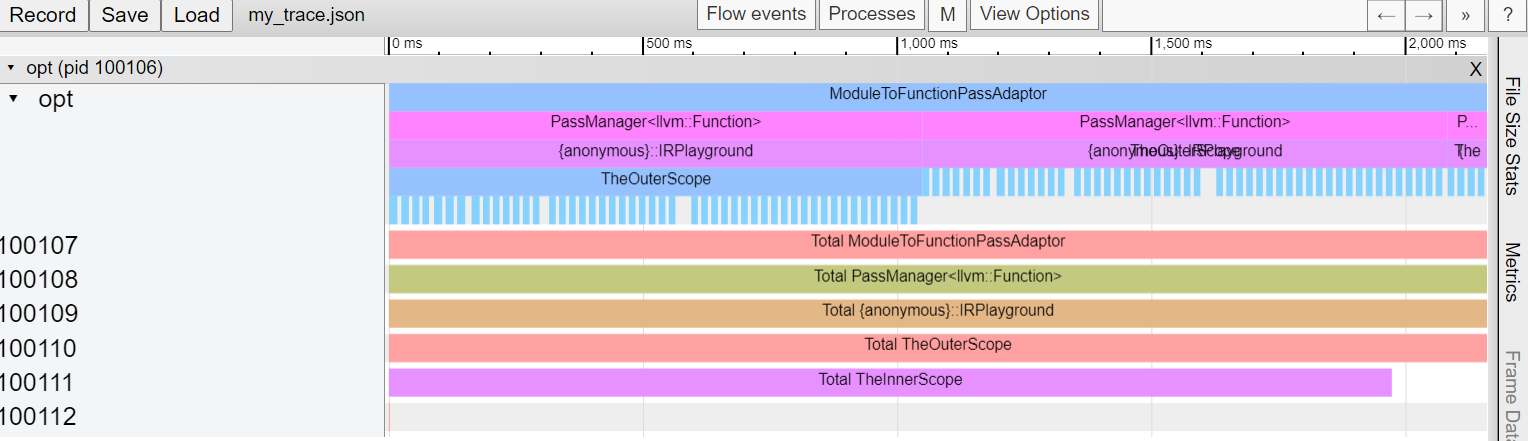
\includegraphics[width=0.9\textwidth]{content/3/chapter11/images/4.png}\\
Figure 11.4 – The view after opening my\_trace.json
\end{center}

Each color block represents a time interval collected by a TimeTraceScope instance.

\item Let's take a closer look: please press the number key 3 to switch to zoom mode. After that, you should be able to zoom in or out by clicking and dragging the mouse up or down. In the meantime, you can use the arrow keys to scroll the timeline left or right. Here is part of the timeline after we zoom in:

\hspace*{\fill} \\ %插入空行
\begin{center}
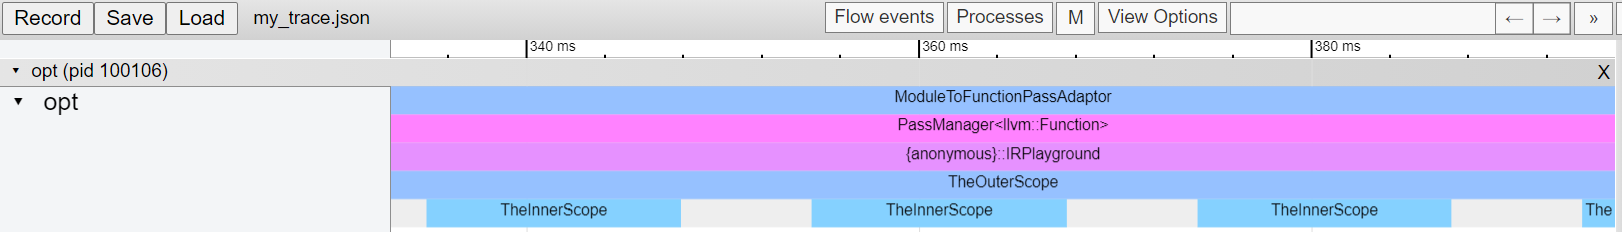
\includegraphics[width=0.9\textwidth]{content/3/chapter11/images/5.png}\\
Figure 11.5 – Part of the trace timeline
\end{center}

As we can see from Figure 11.5, there are several layers stacking together. This layout reflects how different TimeTraceScope instances are organized in opt (and in our Pass). For example, our TimeTraceScope instance entitled TheOuterScope is stacked above multiple TheInnerScope blocks. Each of the TheInnerScope blocks represents the time spent on the foo function in each loop iteration we saw earlier.

\item We can further inspect the properties of a block by clicking on it. For example, if we click one of the TheInnerScope blocks, its timing properties will be shown in the lower half of the screen. Here is an example of this:

\hspace*{\fill} \\ %插入空行
\begin{center}
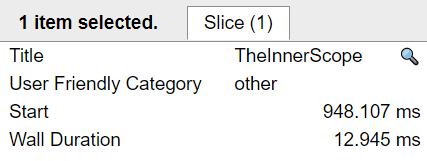
\includegraphics[width=0.9\textwidth]{content/3/chapter11/images/6.png}\\
Figure 11.6 – Details of a time interval block
\end{center}

This gives us information such as the time interval and the starting time in this timeline.

\end{enumerate}

With this visualization, we can combine timing information with the structure of the compiler, which will help us to find out performance bottlenecks more rapidly. 

In addition to opt, clang can also generate the same trace JSON file. Please consider adding a -ftime-trace flag. Here is an example of this:

\begin{tcblisting}{commandshell={}}
$ clang -O3 -ftime-trace -c foo.c
\end{tcblisting}

This will generate a JSON trace file with the same name as the input file. In this case, it will be foo.json. You can use the skills we just learned to visualize it.

In this section, we have learned some useful skills to collect statistics from LLVM. The Statistic class can be used as an integer counter to record the number of events occurring in the optimization. Optimization remarks, on the other hand, can give us insights into some of the decision-making process inside the optimization Pass, making it easier for compiler developers to diagnose missing optimization  opportunities. With Timer and TimeTraceScope, developers can monitor LLVM's execution time in a more manageable way and handle compilation-speed regressions with confidence. These techniques can improve an LLVM developer's productivity when creating new inventions or fixing a challenging problem.

In the next section of this chapter, we are going to learn how to write error-handling code in an efficient way, using utilities provided by LLVM.





